\documentclass{standalone}
\usepackage{tikz}
\usetikzlibrary{shapes.geometric, arrows, positioning, fit, backgrounds, arrows.meta, calc}
\usepackage{tcolorbox}

\tikzstyle{startstop} = [rectangle, rounded corners, 
minimum width=3cm, 
minimum height=1cm,
text centered, 
draw=black, 
fill=red!30]

\tikzstyle{io} = [trapezium, 
trapezium stretches=true, % A later addition
trapezium left angle=70, 
trapezium right angle=110, 
minimum width=3cm, 
minimum height=1cm, text centered, 
draw=black]

\tikzstyle{process} = [rectangle, 
minimum width=3cm, 
minimum height=1cm, 
text centered, 
text width=3cm, 
draw=black]

\tikzstyle{decision} = [diamond, 
minimum width=3cm, 
minimum height=1cm, 
text centered, 
draw=black]
\tikzstyle{arrow} = [thick,->,>=stealth]
\begin{document}

% \begin{tcolorbox}
% \begin{tabular}{ll}
%     \multicolumn{2}{l}{\textbf{Start}}\\
%     P1.     & Operator inserts control mode\\
%     P2      & System checks control mode input\\
%             & \textbf{IF autoMode THEN}\\
%             & \hspace{2mm} P3.A test
% \end{tabular}
% \end{tcolorbox}




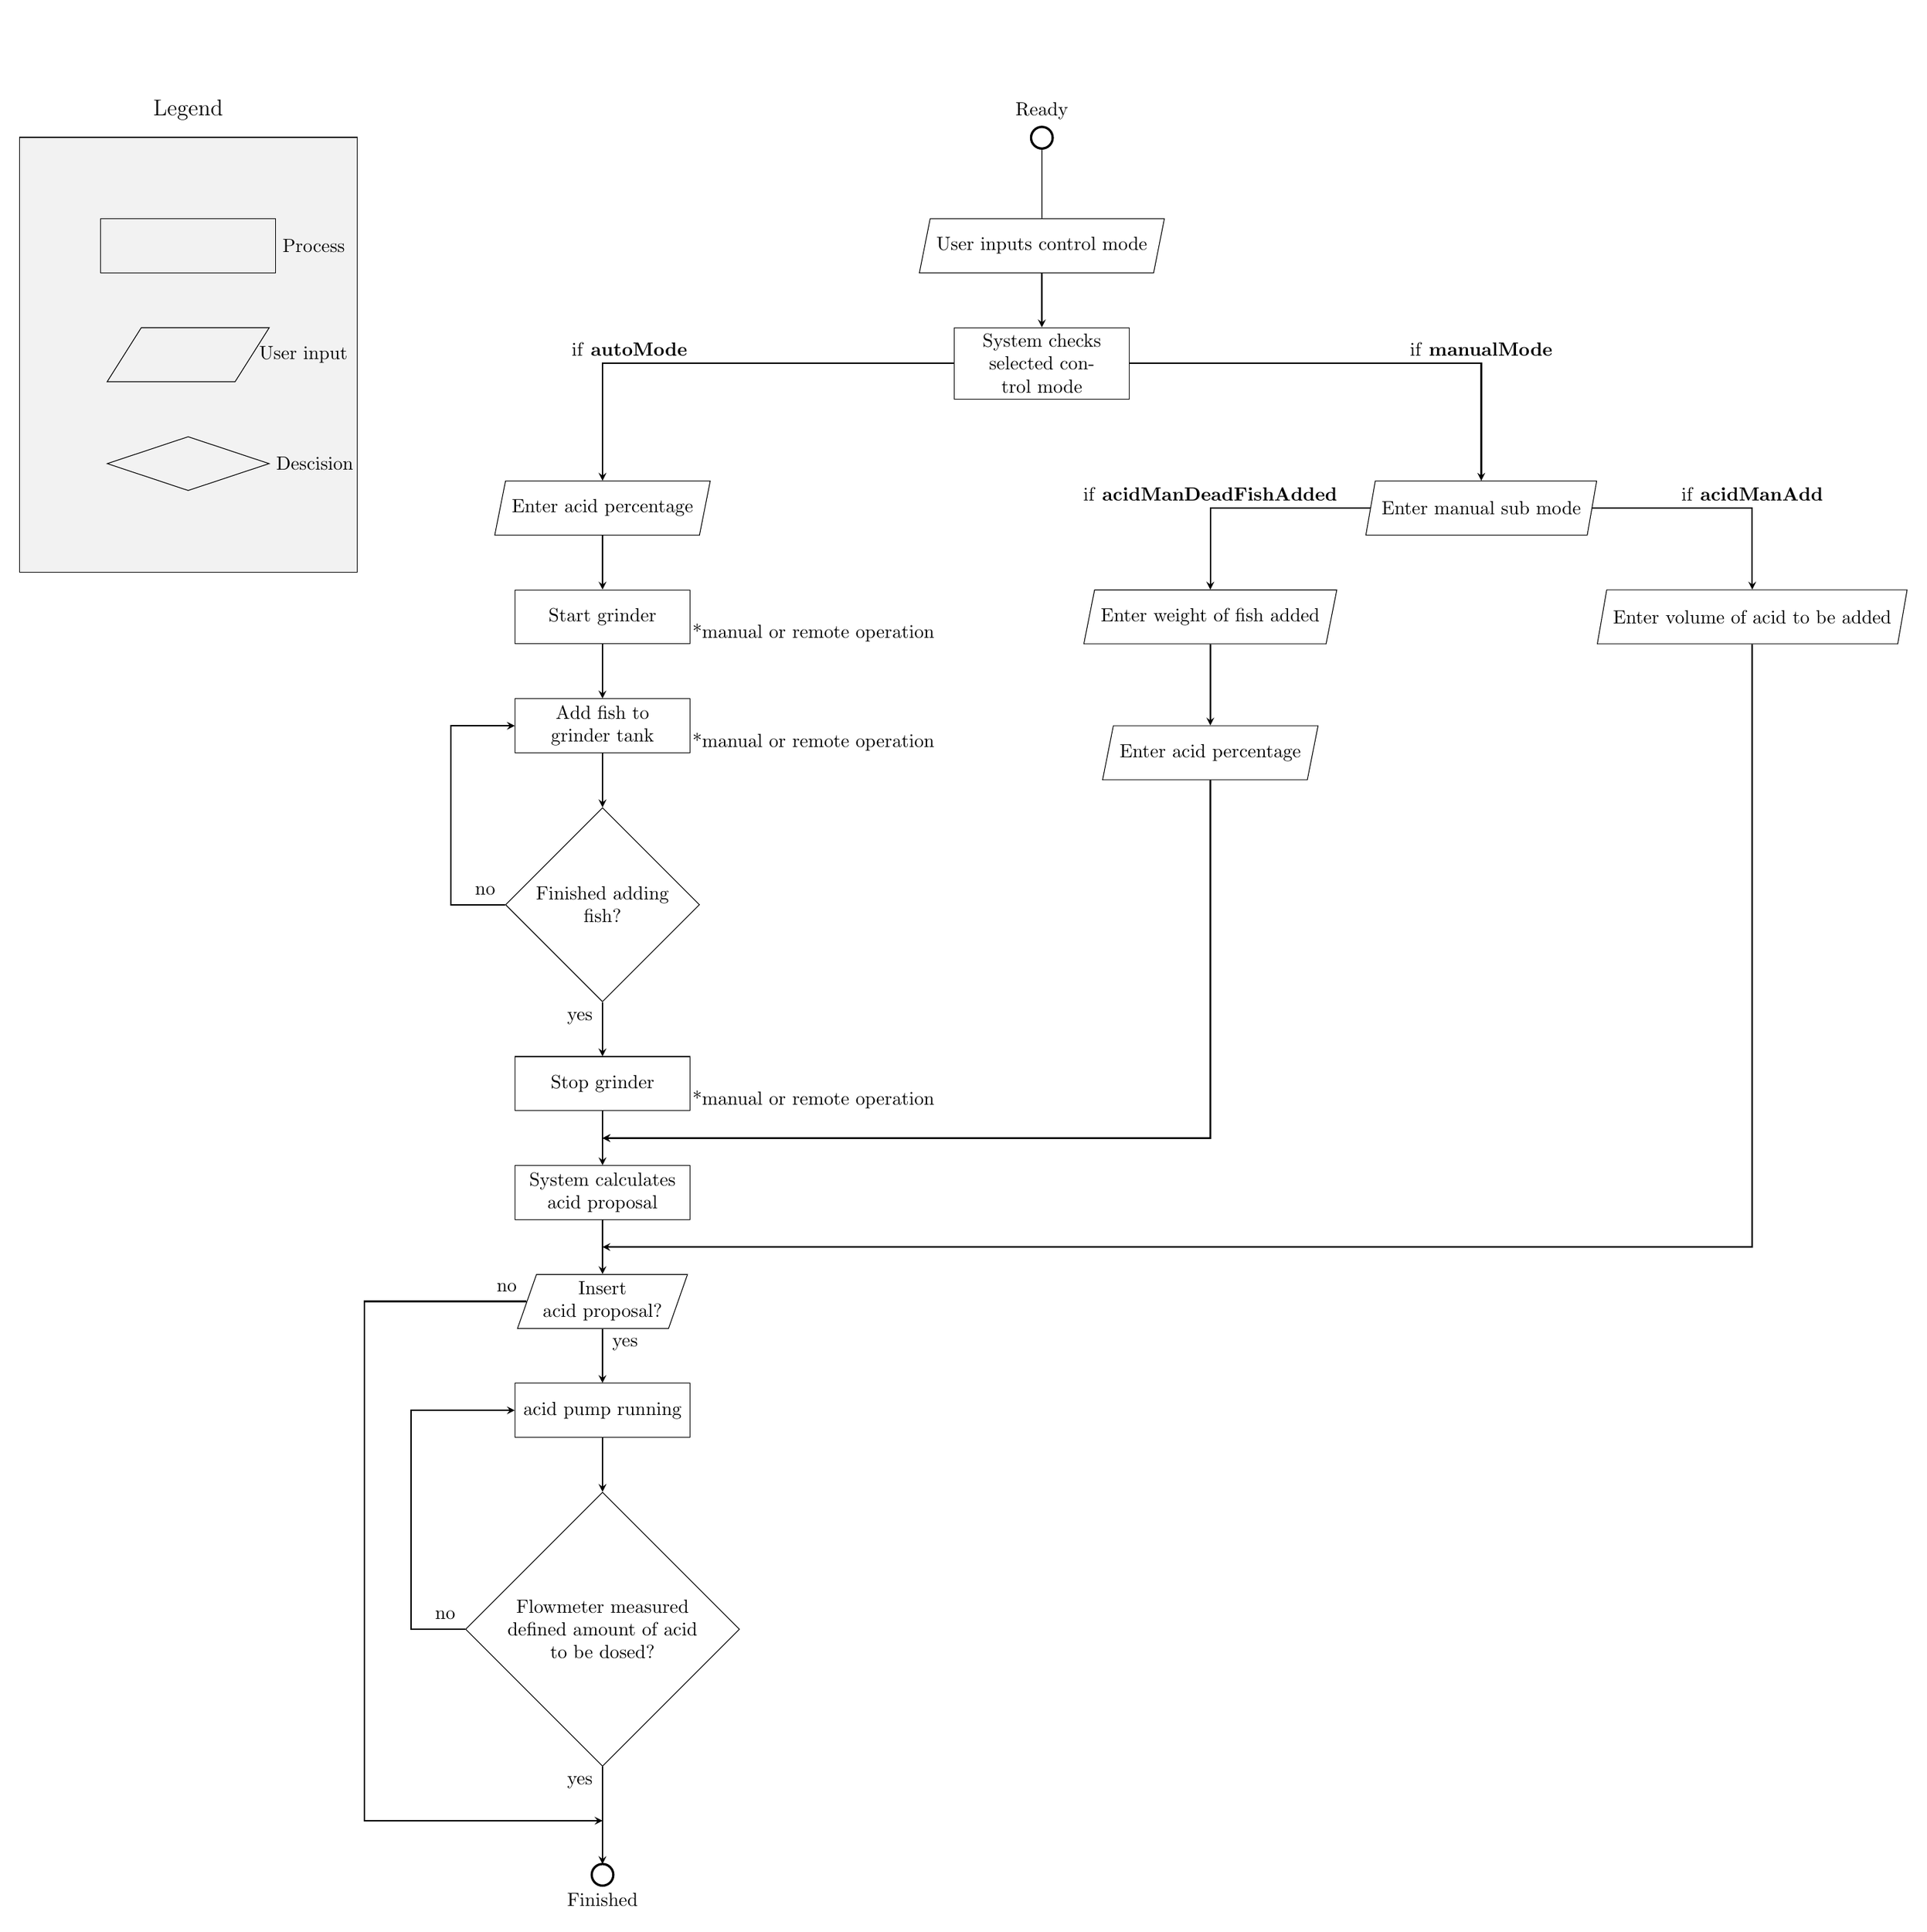
\begin{tikzpicture}[node distance=2cm]


\draw[color=black, very thick](0,0) circle (0.2) node[above=0.2cm] {Ready};
\node (P1) [io] at (0,-2) {User inputs control mode};
\node (d1) [process, below = 1cm of P1] {System checks selected control mode};
\node (P3A) [io, below left = 1cm and 6cm of d1, yshift=-0.5cm] {Enter acid percentage};
\node (P3B) [io, below right = 1cm and 6cm of d1, yshift=-0.5cm] {Enter manual sub mode};
\node (P4A) [process, below = 1cm of P3A] {Start grinder};
\node[anchor=south west,inner sep=1pt, align=left] at (P4A.south east) 
    {*manual or remote operation};
\node (P5A) [process, below = 1cm of P4A] {Add fish to grinder tank};
\node[anchor=south west,inner sep=1pt, align=left] at (P5A.south east) 
    {*manual or remote operation};
\node (d2) [decision, below = 1cm of P5A, align=center] {Finished adding\\fish?};
\node[anchor=south east,inner sep=5pt, align=left] at (d2.west) 
    {no};
\node[anchor=north east,inner sep=5pt, align=left] at (d2.south) 
    {yes};
\node (P6A) [process, below = 1cm of d2] {Stop grinder};
\node[anchor=south west,inner sep=1pt, align=left] at (P6A.south east) 
    {*manual or remote operation};
\node (P7A) [process, below = 1cm of P6A] {System calculates acid proposal};
\node (d3) [io, below = 1cm of P7A, align=center] {Insert\\acid proposal?};
\node[anchor=south east,inner sep=5pt, align=left] at (d3.west) {no};
\node[anchor=north west,inner sep=5pt, align=left] at (d3.south) {yes};
\node (P8A) [process, below = 1cm of d3] {acid pump running};
\node (d4) [decision, below = 1cm of P8A, align=center] {Flowmeter measured\\defined amount of acid\\to be dosed?};
\node (break1) [coordinate, below = 1cm of d4] {};
\node[anchor=north east,inner sep=5pt, align=left] at (d4.south) 
    {yes};
\node[anchor=south east,inner sep=5pt, align=left] at (d4.west) 
    {no};


\node (P3BA) [io, below left = 1cm and 4cm of P3B] {Enter weight of fish added};
\node (P4MAN) [io, below = 1cm of P3BA, yshift=-0.5cm] {Enter acid percentage};
\node (break2) [coordinate, above = .5cm of P7A] {};
\node (P5MAN) [io, below right = 1cm and 4cm of P3B] {Enter volume of acid to be added};
\node (break3) [coordinate, above = .5cm of d3] {};

%%%%% LEGEND %%%%%%%%%

\node (leg1) [process, left = 12cm of P1,label=right:Process] {};
\node (leg2) [io, below = 1cm of leg1,label=right:User input] {};
\node (leg3) [decision, below = 1cm of leg2,label=right:Descision] {};
\begin{scope}[on background layer,inner sep=1.5cm]
    \node[fill=gray!10,draw,fit=(leg1) (leg2) (leg3),label={[yshift=-1.2cm]\large Legend}] {};
\end{scope}


%%% DRAW %%%
\draw[] (0,-0.2) -- (P1);
\draw [arrow] (P1) -- (d1);
\draw [arrow] (d1) -| node[midway, above, xshift=0.5cm]{if \textbf{autoMode}} (P3A);'
\draw [arrow] (d2.west) -- +(-1,0) |- (P5A.west);
\draw [arrow] (d2) -- (P6A);
\draw [arrow] (P3A) -- (P4A);
\draw [arrow] (P4A) -- (P5A);
\draw [arrow] (P5A) -- (d2);
\draw [arrow] (P6A) -- (P7A);
\draw [arrow] (P7A) -- (d3);
\draw [arrow] (d3) -- (P8A);
\draw [arrow] (d3.west) -- +(-3,0) |- (break1);
\draw [arrow] (P8A) -- (d4);
\draw[color=black, very thick](d4.south)[yshift=-2cm] circle (0.2) node[below=0.2cm] {Finished};
\draw [arrow] (d4.south) -- +(0,-1.8);
\draw [arrow] (d4.west) -- +(-1,0) |- (P8A.west);

\draw [arrow] (d1) -| node[above, midway]{if \textbf{manualMode}} (P3B);'
\draw [arrow] (P3B)-| node[midway, above]{if \textbf{acidManDeadFishAdded}} (P3BA);
\draw [arrow] (P4MAN) -- +(0,-2) |- (break2);
\draw [arrow] (P4MAN) -- +(0,-2) |- (break2);
\draw [arrow] (P3BA) -- (P4MAN);
\draw [arrow] (P3B)-| node[midway, above]{if \textbf{acidManAdd}} (P5MAN);
\draw [arrow] (P5MAN) -- +(0,-2) |- (break3);


% \draw [arrow] (start) -- (in1);
% \draw [arrow] (in1) -- (pro1);
% \draw [arrow] (pro1) -- (dec1);
% \draw [arrow] (dec1) -- node[anchor=east] {yes} (pro2a);
% \draw [arrow] (dec1) -- node[anchor=south] {no} (pro2b);
% \draw [arrow] (pro2b) |- (pro1);
% \draw [arrow] (pro2a) -- (out1);
% \draw [arrow] (out1) -- (stop);

\end{tikzpicture}
\end{document}